\documentclass[aps,pra,notitlepage,amsmath,amssymb,letterpaper,12pt]{revtex4-1}
\usepackage{amsthm}
\usepackage{graphicx}
%  Above uses the Americal Physical Society template for Physical Review A
%  as a reasonable and fully-featured default template
 
%  Below define helpful commands to set up problem environments easily
\newenvironment{problem}[2][Problem]{\begin{trivlist}
\item[\hskip \labelsep {\bfseries #1}\hskip \labelsep {\bfseries #2.}]}{\end{trivlist}}
\newenvironment{solution}{\begin{proof}[Solution]}{\end{proof}}
 
% --------------------------------------------------------------
%                   Document Begins Here
% --------------------------------------------------------------
 
\begin{document}
 
\title{Definition of a Derivative}
\author{Sharon Kim, Kynan Barton, Kristalee Lio}
\affiliation{CS 510, Schmid College of Science and Technology, Chapman University}
\date{\today}



\section{The Derivative}



Let $y = f(x)$ be a function. The derivative of f is the function whose value at x is the limit provided this limit exists.


\begin{align}
f'(x) &= \lim_{h \to 0} \frac{f(x+h)-f(x)}{h}.
\end{align}




If this limit exists for each x in an open interval I, then we say that f is differentiable on I.













Figures can be included easily.

\begin{figure}[h!] % h forces the figure to be placed here, in the text
 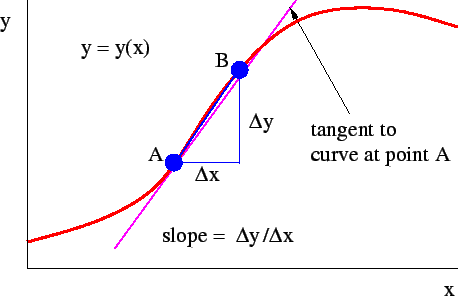
\includegraphics[width=0.4\textwidth]{Introductory_Physics_fig_1_15.png}  % if pdflatex is used, jpg, pdf, and png are permitted
  \caption{The figure caption goes here.}
  \label{fig:figlabel}
\end{figure}

This text should be below the figure unless \LaTeX  decides that a different layout works better.
 

 
\end{document}
